\chapter{Конструкторский раздел}

В данном разделе представлены схемы реализуемых алгоритмов и их модификации.

\section{Трудоемкость алгоритмов}\label{estimate}
Для получения функции трудоемкости алгоритма необходимо ввести модель оценки трудоемкости. Трудоемкость "элементарных" операций оценивается следующим образом:
\begin{enumerate}
	\item Трудоемкость 1 имеют операции:
	\begin{equation*}\label{math:simple}
		\begin{array}{cc}
			+, -, =, <, >, <=, >=, ==, +=, -=,\\
			++, --, [], \&\&, ||, >>, << \\
		\end{array}
	\end{equation*}
	\item Трудоемкость 2 имеют операции:
	\begin{equation*}\label{math:complex}
		*, /, \char`\\ , \%
	\end{equation*}	
	\item Трудоемкость конструкции ветвления определяется согласно формуле \ref{math:if}.
	\begin{equation}\label{math:if}
		f_{if} = f_{\text{условие}} + 
		\begin{sqcases}
			min\left(f_{true} , f_{false}\right) \text{ в лучшем случае,} \\
			max\left(f_{true} , f_{false}\right) \text{ в худшем случае.} \\
		\end{sqcases}
	\end{equation}
	\item Трудоемкость цикла расчитывается по формуле \ref{math:loop}.
	\begin{equation}\label{math:loop}
		f_{\text{цикл}} = f_{\text{инициализация}} + f_{\text{сравнение}} + N \left(f_{\text{тело}} + f_{\text{инкремент}} + f_{\text{сравнение}}\right);
	\end{equation}
	\item Трудоемкость вызова функции равна 0.
\end{enumerate}

\section{Трудоемкость алгоритмов}

\subsection{Алгоритм сортировки бинарным деревом}

Трудоёмкость данного алгоритма посчитаем следующим образом: сортировка -- преобразование массива в бинарное дерево поиска посредством операции вставки нового элемента в бинарное дерево.
Операция вставки в бинарное дерево имеет сложность $ \log_{2}(size)$, где $size$ - количество элементов в дереве.
Для преобразования массива или списка размером $size$ потребуется использовать операцию вставки в биннарное дерево $size$ раз, таким образом, итоговая трудоёмкость данной сортировки будет равна (\ref{for:binary_sort_perf}):
\begin{align}
	\begin{split}
		\label{for:binary_sort_perf}
		f_{radix} &= size \cdot \log_{2}(size);
	\end{split}
\end{align}


\subsection{Алгоритм сортировки подсчетом}

Трудоёмкость алгоритма сортировки подсчётом, где size --- количество элементов в массиве (\ref{for:count_sort_perf}):
\begin{align}
	\begin{split}
		\label{for:count_sort_perf}
		f_{count} &= size + 10  + 2 + size \cdot 8 + 2 + 10 \cdot 6 + 3 \\
		&+ size \cdot 14 + 1 + size \cdot 5 \\
		&= 78 + 28 \cdot size = O(n);
	\end{split}
\end{align}

\subsection{Алгоритм поразрядной сортировки}

Трудоёмкость алгоритма поразрядной сортировки равна %(\ref{for:radix_sort_perf}):
\begin{align}
	\label{for:radix_sort_perf}
	f_{radix} = 1 + 2 + 5 \cdot size + 1 + 2 + m * (f_{count} + 1 + 2);
\end{align}
где $m$ - количество разрядов в максимальном элементе, $f_{count}$ - трудоёмкость алгоритма сортировки подсчётом.

Итоговая трудоёмкость порязрядной сортировки, использующей сортировку подсчётом в рамках одного разряда: 
\begin{align}
	f_{radix} = 28 \cdot m \cdot size = O(n);
\end{align}

\section{Схемы алгоритмов}
На рисунке \ref{fig:alg} приведена схема алгоритма сортировки бинарным деревом. На рисунке \ref{fig:win-1} приведена схема алгоритма сортировки подсчетом. Рисунок  
\ref{fig:win-2} демонстрируют схему алгоритма поразряндной сортировки.\newpage

\begin{figure}[ht!]
	\centering
	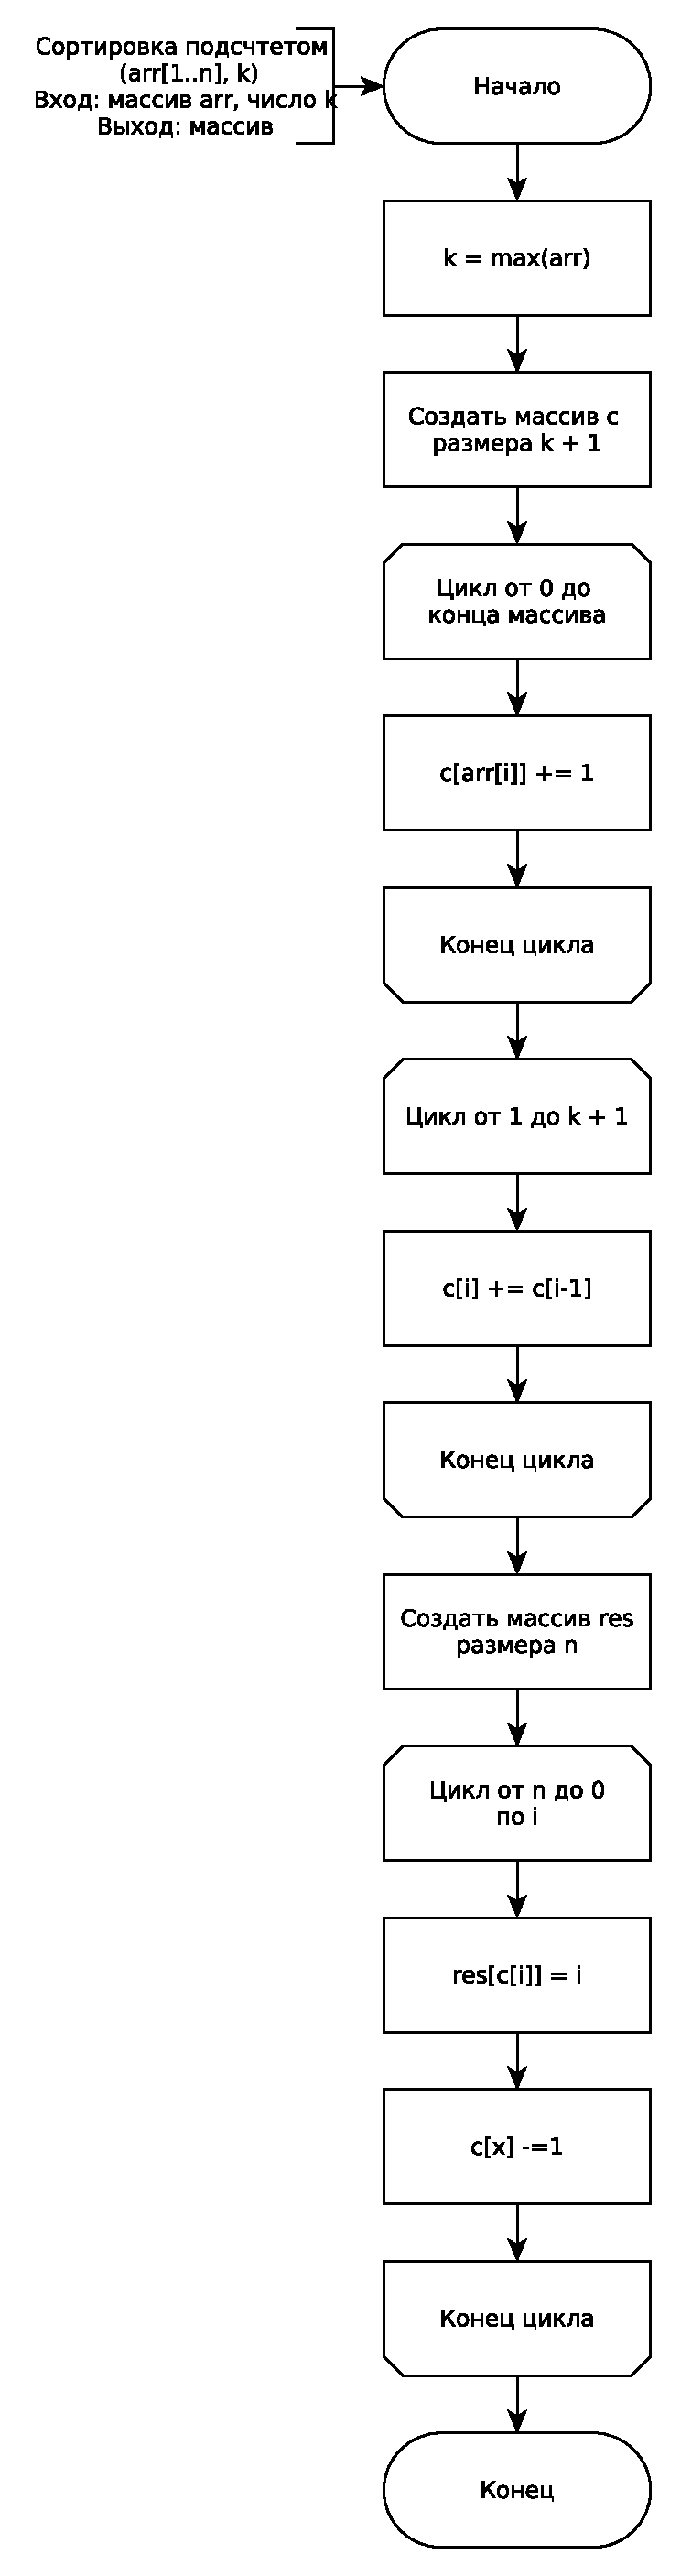
\includegraphics[width=0.45\linewidth]{assets/count.pdf}
	\caption{Схема алгоритма сортировки подсчетом}
	\label{fig:win-1}
\end{figure}

\begin{figure}[ht!]
	\centering
	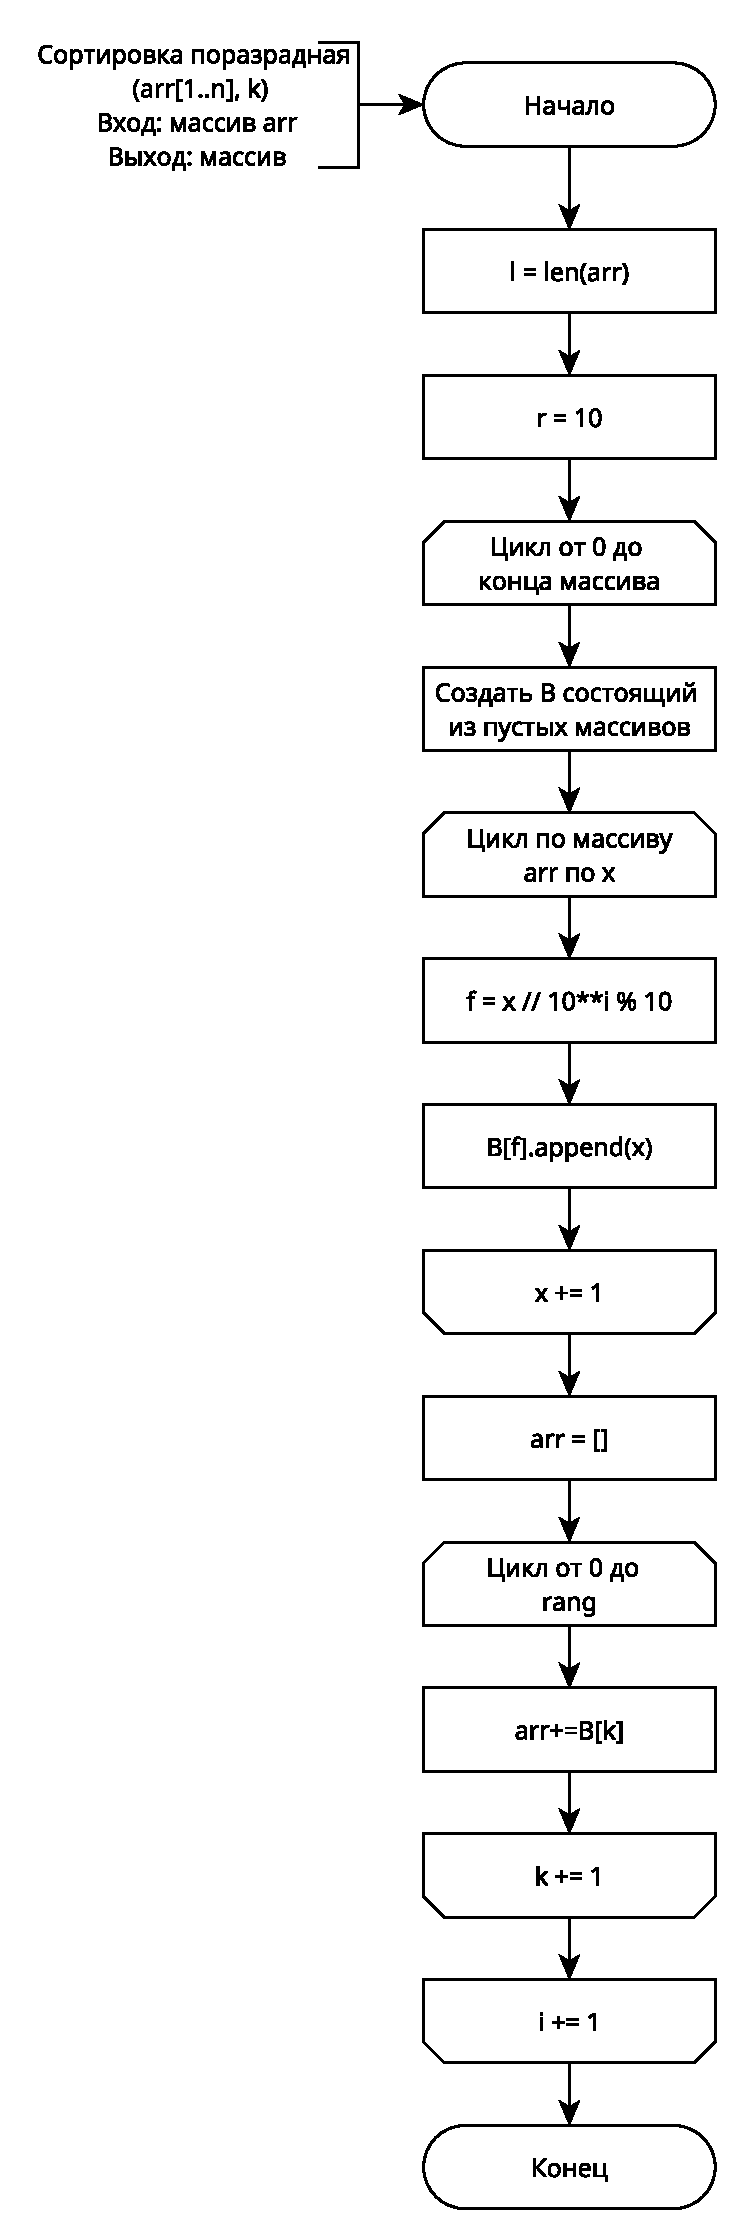
\includegraphics[width=0.47\linewidth]{assets/range.pdf}
	\caption{Схема алгоритма поразряндной сортировки}
	\label{fig:win-2}
\end{figure}

\begin{figure}[ht!]
	\centering
	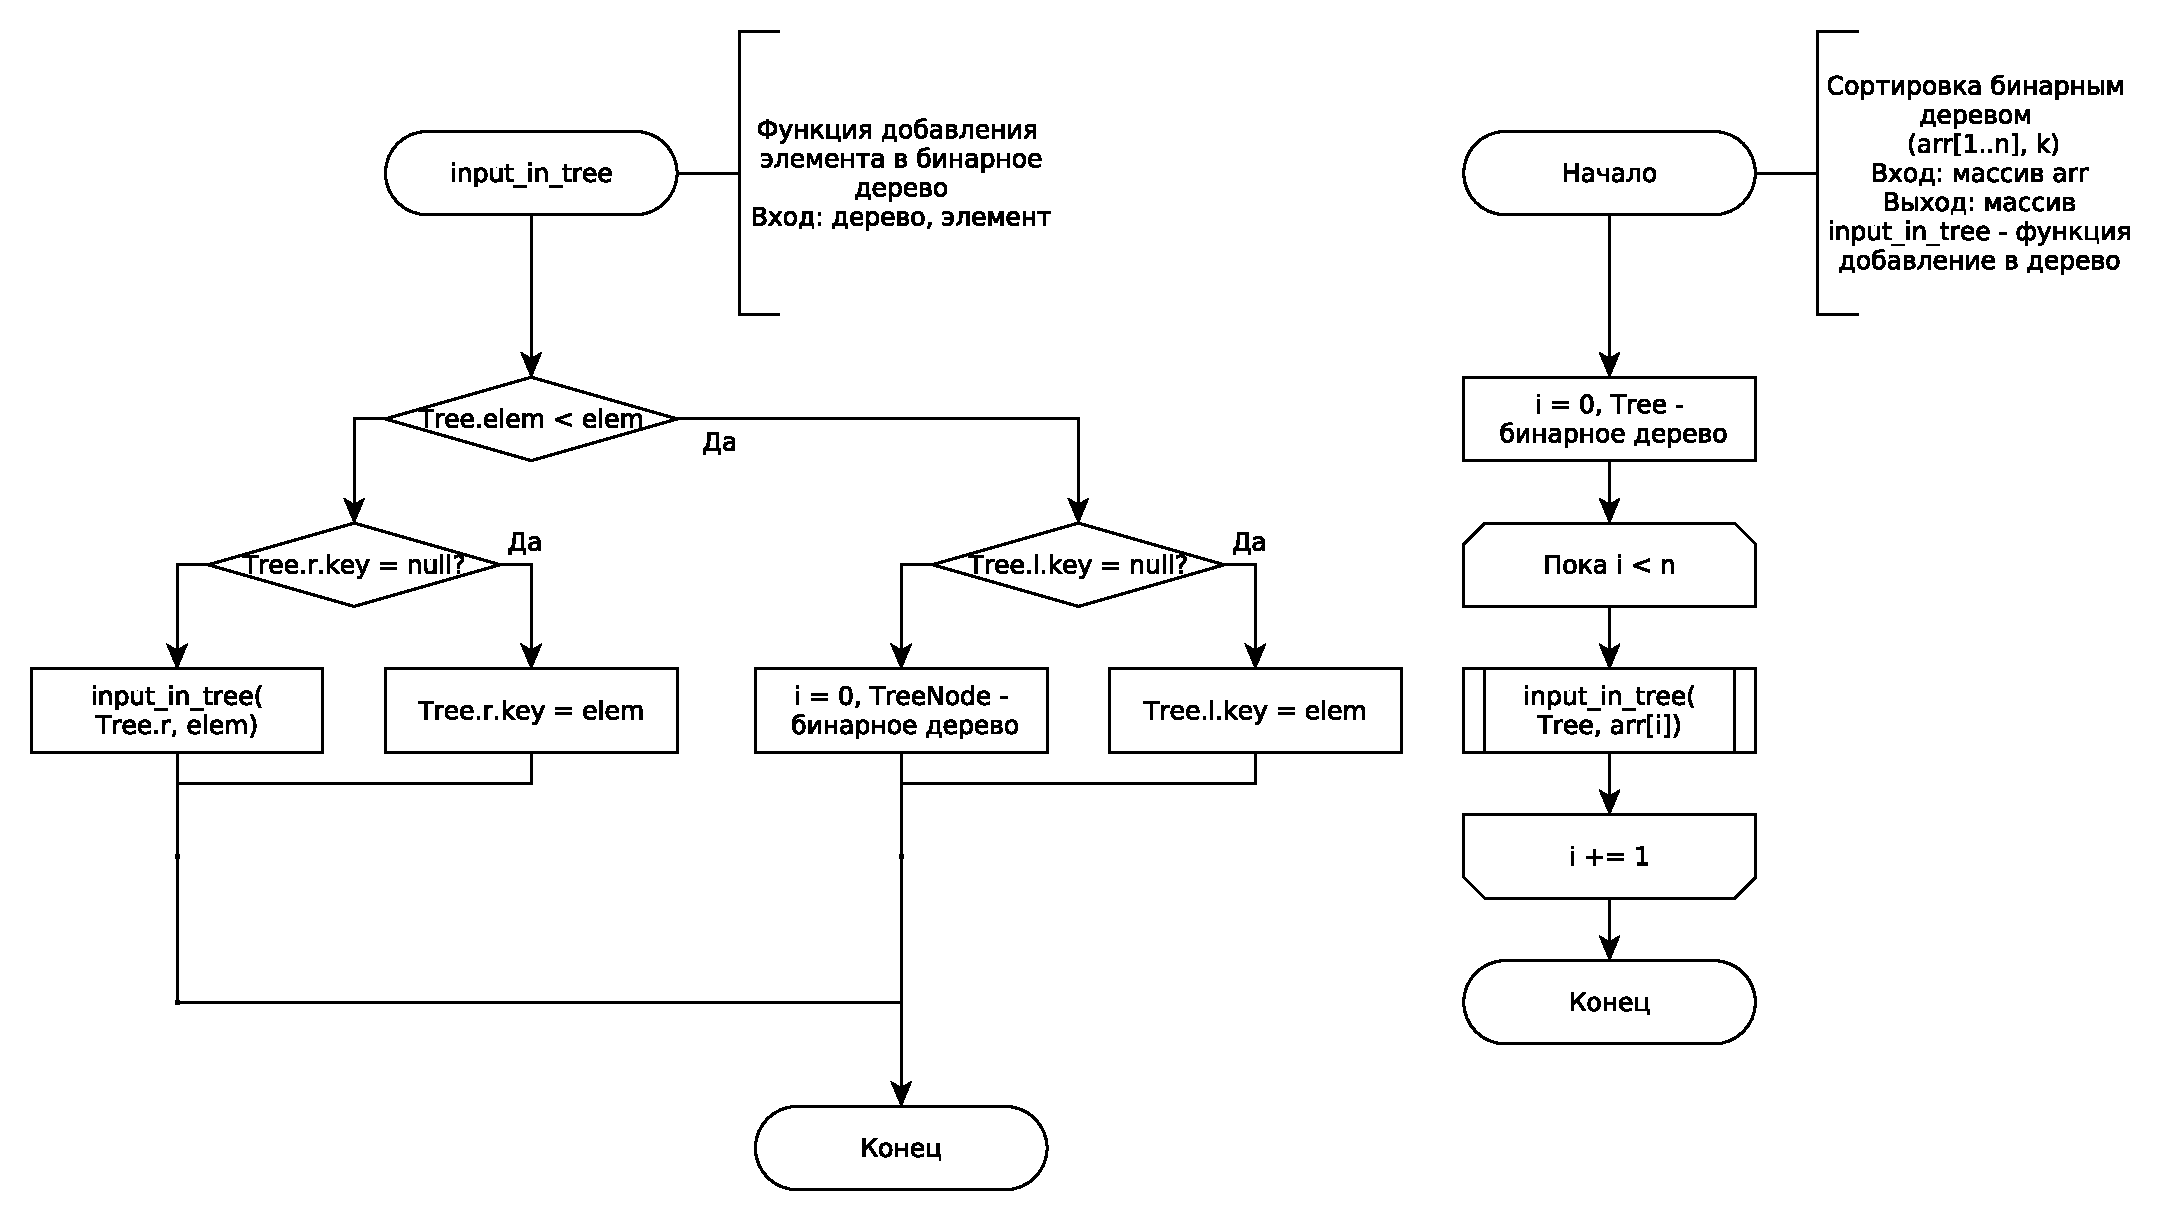
\includegraphics[width=1\linewidth]{assets/bintree.pdf}
	\caption{Схема алгоритма сортировки бинарным деревом}
	\label{fig:alg}
\end{figure}



\section*{Вывод}
Были разработаны схемы всех трех алгоритмов сортировки. Также для каждого из них были рассчитаны трудоёмкости по введённой модели вычислений с учётом лучших и худших случаев.